\chapter{Luchtdruk en weer}\label{ch:g5:air-pressure-weather}

Je woont op de bodem van een oceaan --- een oceaan van \omterm{def:g2:air-around-us:air}{lucht},
honderden kilometers diep, met het hele \omterm{def:g4:weight-and-mass:weight}{gewicht} ervan op je
schouders. Waarom verplettert die je niet? Waarom voel je hem niet
eens? En wat heeft dit allemaal met het weer van morgen te maken?
\omterm{def:g2:air-around-us:air}{Lucht}, onze oude onzichtbare vriendin, heeft nog één groot geheim
prijs te geven.

\section{Lucht heeft gewicht}

\begin{example}[Het onzichtbare wegen]\label{ex:g5:air-pressure-weather:weighing}
Een stevige voetbal wordt op een fijne \omterm{def:g3:levers-and-scales:scale}{balansweegschaal} gelegd en
precies in \omterm{def:g2:balance-equilibrium:equilibrium}{evenwicht} gebracht. Dan gaat het ventiel open en sist de
extra \omterm{def:g2:air-around-us:air}{lucht} eruit --- dezelfde bal, hetzelfde ventiel, alles hetzelfde,
op wat \omterm{def:g2:air-around-us:air}{lucht} na. Terug op de weegschaal: de leeggelopen bal is
\emph{lichter}. Het verschil is het \omterm{def:g4:weight-and-mass:weight}{gewicht} van de ontsnapte
\omterm{def:g2:air-around-us:air}{lucht}. \omterm{def:g2:air-around-us:air}{Lucht} is stof, stof heeft \omterm{def:g3:measuring-mass:mass}{massa}, en \omterm{def:g3:measuring-mass:mass}{massa} wordt door de
Aarde omlaag getrokken: de oceaan boven ons is zwaar.
\end{example}

\begin{definition}[De dampkring en zijn druk]\label{def:g5:air-pressure-weather:pressure}
De \emph{dampkring}\index{dampkring} is de diepe laag \omterm{def:g2:air-around-us:air}{lucht} die om de
hele Aarde gewikkeld zit. Zijn \omterm{def:g4:weight-and-mass:weight}{gewicht} perst de \omterm{def:g2:air-around-us:air}{lucht} onderin samen
--- daar waar wij wonen --- en samengeperste \omterm{def:g2:air-around-us:air}{lucht} duwt hard tegen elk
oppervlak dat ze raakt. Die duw heet
\emph{luchtdruk}\index{luchtdruk}.
\end{definition}

\begin{proposition}[De duw van alle kanten]\label{prop:g5:air-pressure-weather:allsides}
\omterm{def:g5:air-pressure-weather:pressure}{Luchtdruk} duwt op elk oppervlak vanuit \emph{elke} richting ---
omlaag op tafels, zijwaarts op muren, en zelfs \emph{omhoog} op
plafonds en handpalmen. En ze is machtig: op een oppervlak zo groot
als je handpalm duwt de \omterm{def:g2:air-around-us:air}{lucht} ongeveer zo hard als het \omterm{def:g4:weight-and-mass:weight}{gewicht} van
een grote, volle koffer. We merken het nooit, doordat de duwen in
\omterm{def:g2:balance-equilibrium:equilibrium}{evenwicht} komen: de \omterm{def:g2:air-around-us:air}{lucht} in ons en achter elk oppervlak duwt precies
zo hard terug.
\end{proposition}

\begin{method}[Het kaartje dat water tegenhoudt]\label{met:g5:air-pressure-weather:card}
De duw van de \omterm{def:g2:air-around-us:air}{lucht} omhoog, op heterdaad betrapt (doe het boven de
gootsteen):
\begin{enumerate}
  \item vul een glas tot aan de rand met water;
  \item leg er een stevig, glad kaartje plat bovenop, dat het water
        rondom raakt;
  \item houd het kaartje op zijn plaats, keer het glas precies
        ondersteboven en laat het kaartje voorzichtig los.
\end{enumerate}
Het kaartje blijft zitten --- en houdt het hele glas vol tegen. Het
\omterm{def:g4:weight-and-mass:weight}{gewicht} van het water drukt op het kaartje omlaag, maar de
\omterm{def:g5:air-pressure-weather:pressure}{dampkring} drukt er nog harder \emph{omhoog} tegen. Je hebt zojuist
de koffer-duw van onderaf gezien.
\end{method}

\begin{omfigure}
\begin{tikzpicture}[scale=0.85]
  \draw[thick] (4.4,1.2) -- (4.4,3.6) (6.6,1.2) -- (6.6,3.6);
  \draw[thick] (4.4,3.6) -- (6.6,3.6);
  \fill[omDef, opacity=0.25] (4.4,1.25) rectangle (6.6,3.55);
  \draw[very thick, omMeth] (4.25,1.2) -- (6.75,1.2);
  \node[right, font=\small, omMeth] at (6.9,1.2) {het kaartje};
  \draw[-Stealth, thick, omDef] (5.0,2.9) -- (5.0,2.2);
  \draw[-Stealth, thick, omDef] (6.0,2.9) -- (6.0,2.2);
  \node[above, font=\small, omDef] at (5.5,3.65)
    {water duwt omlaag};
  \foreach \x in {4.7,5.5,6.3} {
    \draw[-Stealth, very thick, omThm] (\x,0.15) -- (\x,0.95);
  }
  \node[below, font=\small, omThm] at (5.5,-0.05)
    {de dampkring duwt omhoog --- harder};
\end{tikzpicture}

{\small Het omgekeerde glas: de duw van de \omterm{def:g2:air-around-us:air}{lucht} omhoog tegen het
kaartje is sterker dan het \omterm{def:g4:weight-and-mass:weight}{gewicht} van het water. De onzichtbare oceaan
is sterk.}
\end{omfigure}

\section{Machines die op de dampkring draaien}

\begin{example}[Het rietje]\label{ex:g5:air-pressure-weather:straw}
Je denkt dat je sap door een rietje omhoog trekt. In werkelijkheid kun
je een \omterm{def:g3:solids-liquids-gases:liquid}{vloeistof} helemaal niet trekken --- probeer maar eens water met
je vingers te trekken! Wat je werkelijk doet, is de \emph{\omterm{def:g2:air-around-us:air}{lucht}} uit
het rietje zuigen. Met de \omterm{def:g2:air-around-us:air}{lucht} weg van binnen duwt de \omterm{def:g5:air-pressure-weather:pressure}{dampkring},
die op het sap in het glas drukt, het sap door het lege rietje omhoog
je mond in. Elke slok is de \omterm{def:g5:air-pressure-weather:pressure}{dampkring} die het tilwerk doet; jij maakt
alleen de weg vrij.
\end{example}

\begin{example}[Zuignappen en ingedeukte flessen]\label{ex:g5:air-pressure-weather:suction}
De rubberen nap van het badkamerhaakje wordt plat tegen de tegels
gedrukt, waarbij de \omterm{def:g2:air-around-us:air}{lucht} eronder vandaan wordt geperst: nu duwt de
\omterm{def:g5:air-pressure-weather:pressure}{dampkring} de nap tegen de muur zonder dat er iets achter zit dat
terugduwt --- vastgepind door de hemel zelf. En draai de dop op een
lege plastic fles hoog in de bergen, en rijd dan het dal in: de fles
kreukelt alsof een spookhand hem samenknijpt. Buiten drukt meer
\omterm{def:g2:air-around-us:air}{lucht} dan de ijle bergluchtlucht die binnenin is opgesloten --- de
\omterm{def:g5:air-pressure-weather:pressure}{dampkring} wint, en de fles vouwt in.
\end{example}

\begin{example}[IJler met de hoogte]\label{ex:g5:air-pressure-weather:height}
Klim, en je laat een deel van de oceaan onder je: minder \omterm{def:g2:air-around-us:air}{lucht}
erboven betekent een zwakkere duw. Je oren klappen in een snelle
kabelbaan terwijl de druk buiten verandert; bergbeklimmers happen naar
ijl geworden \omterm{def:g2:air-around-us:air}{lucht}. En hier geeft het bergtheeraadsel van vorig jaar
zich over: doordat de \omterm{def:g5:air-pressure-weather:pressure}{dampkring} minder op het water drukt, komt het
koken makkelijker --- water kookt op grote toppen ruim onder
\qty{100}{\celsius}, te koel om goed te laten trekken.
\end{example}

\begin{omfigure}
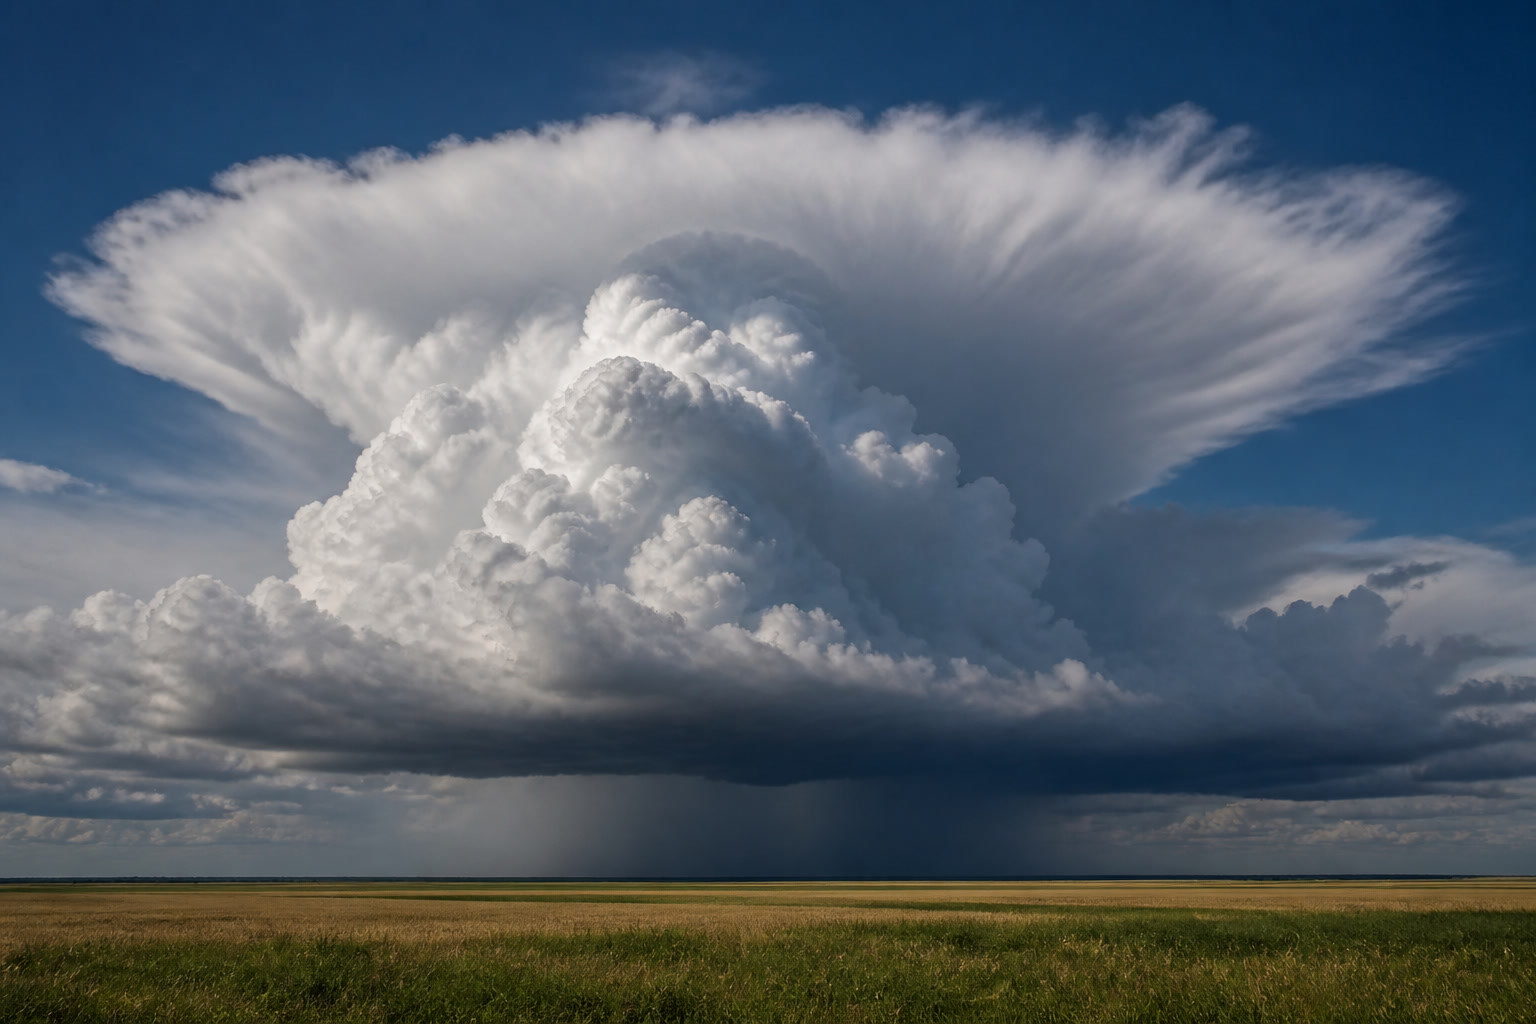
\includegraphics[width=0.58\linewidth]{images/book1/ai/g5-weather-storm.jpg}

{\small Een onweerswolk die boven de velden uittorent: weer is de \omterm{def:g5:air-pressure-weather:pressure}{dampkring} in beweging.}
\end{omfigure}

\section{De barometer en het weer}

\begin{definition}[Barometer]\label{def:g5:air-pressure-weather:barometer}
Een \emph{barometer}\index{barometer} is het instrument dat
\omterm{def:g5:air-pressure-weather:pressure}{luchtdruk} meet --- alweer een lid van onze familie eerlijke
rechters, naast de \omterm{def:g3:temperature-thermometers:temperature}{thermometer} en de weegschaal. Zijn naald stijgt
wanneer de \omterm{def:g5:air-pressure-weather:pressure}{dampkring} erboven harder drukt, en daalt wanneer de druk
lichter wordt.
\end{definition}

\begin{proposition}[De druk praat over morgen]\label{prop:g5:air-pressure-weather:weather}
De druk van de \omterm{def:g5:air-pressure-weather:pressure}{dampkring} is rusteloos: zware, dalende \omterm{def:g2:air-around-us:air}{lucht} brengt
rustige, heldere hemels; lichte, stijgende \omterm{def:g2:air-around-us:air}{lucht} nodigt wolken en
regen uit. De \omterm{def:g5:air-pressure-weather:barometer}{barometer} is dus een waarzegger van bescheiden,
eerlijke soort: \emph{gelijkblijvende of stijgende} druk belooft mooi
weer; \emph{dalende} druk waarschuwt voor wolken op komst; een
\emph{snelle daling} betekent dat er een storm op weg kan zijn.
\end{proposition}

\begin{omfigure}
\begin{tikzpicture}[scale=0.85]
  \draw[thick] (2.2,1.7) circle (1.5);
  \foreach \a/\t in {150/{}, 120/{}, 90/{}, 60/{}, 30/{}} {
    \draw (2.2,1.7) ++(\a:1.3) -- ++(\a:0.18);
  }
  \node[font=\footnotesize] at (1.1,2.6) {regen};
  \node[font=\footnotesize] at (2.2,3.0) {verandering};
  \node[font=\footnotesize] at (3.4,2.6) {mooi weer};
  \draw[-Stealth, very thick, omThm] (2.2,1.7) -- ++(55:1.1);
  \fill (2.2,1.7) circle (2pt);
  \node[below, font=\small] at (2.2,-0.05)
    {een huisbarometer: de naald neigt naar mooi weer};
  \node[right, font=\small, align=left] at (5.4,2.5)
    {stijgende naald: heldere hemel op komst};
  \node[right, font=\small, align=left] at (5.4,1.7)
    {dalende naald: wolken pakken samen};
  \node[right, font=\small, align=left] at (5.4,0.9)
    {snel dalend: alles vastzetten --- storm};
\end{tikzpicture}

{\small Een \omterm{def:g5:air-pressure-weather:barometer}{barometer} aflezen: niet zozeer waar de naald staat als wel
welke kant hij op beweegt --- de \omterm{def:g5:air-pressure-weather:pressure}{dampkring} kondigt zijn plannen aan.}
\end{omfigure}

\begin{remark}[De H en de L op de weerkaart]\label{rem:g5:air-pressure-weather:map}
Het weerbericht van vanavond laat grote wervels zien met H en L
erbij: gebieden van hoge en lage druk die als trage walvissen over de
kaart \omterm{def:g1:floating-and-sinking:words}{drijven}. \omterm{def:g2:air-around-us:air}{Lucht} stroomt onophoudelijk van de zware H-gebieden
naar de lichte L-gebieden --- en dat stromen \emph{is de \omterm{def:g2:air-around-us:wind}{wind}}. Eén
hoofdstuk, drie oude bekenden verklaard: de voorspelling van de
\omterm{def:g5:air-pressure-weather:barometer}{barometer}, de oorsprong van de \omterm{def:g2:air-around-us:wind}{wind}, en de reden waarom je oren
weten wanneer het weer gaat omslaan.
\end{remark}

\section{Oefeningen}

\begin{exercise}[$\star$]\label{exo:g5:air-pressure-weather:1}
Hoe laat de voetbalproef zien dat \omterm{def:g2:air-around-us:air}{lucht} \omterm{def:g4:weight-and-mass:weight}{gewicht} heeft? Wat wordt er
precies vergeleken?
\end{exercise}

\begin{exercise}[$\star$]\label{exo:g5:air-pressure-weather:2}
Wat is \omterm{def:g5:air-pressure-weather:pressure}{luchtdruk}, en waar komt ze vandaan? In welke richtingen duwt
ze?
\end{exercise}

\begin{exercise}[$\star$]\label{exo:g5:air-pressure-weather:3}
De \omterm{def:g5:air-pressure-weather:pressure}{dampkring} drukt op je handpalm ongeveer zo hard als een volle
koffer weegt --- en toch voel je niets. Waarom niet?
\end{exercise}

\begin{exercise}[$\star$]\label{exo:g5:air-pressure-weather:4}
Bij de kaartjestruc strijden twee duwen om het kaartje. Noem ze, en
zeg welke wint.
\end{exercise}

\begin{exercise}[$\star$]\label{exo:g5:air-pressure-weather:5}
``Ik trek het sap door het rietje omhoog.'' Verbeter deze zin: wat
haal je werkelijk weg, en wie doet het tilwerk?
\end{exercise}

\begin{exercise}[$\star$]\label{exo:g5:air-pressure-weather:6}
Waarom klemt een zuignap zich aan de tegels vast? Wat is er
weggeperst, en wat houdt de nap vast?
\end{exercise}

\begin{exercise}[$\star$]\label{exo:g5:air-pressure-weather:7}
Wat gebeurt er met de \omterm{def:g5:air-pressure-weather:pressure}{luchtdruk} als je een berg beklimt, en waarom?
Geef twee tekenen ervan die een reiziger kan opmerken.
\end{exercise}

\begin{exercise}[$\star$]\label{exo:g5:air-pressure-weather:8}
Wat meet een \omterm{def:g5:air-pressure-weather:barometer}{barometer}? Jouw \omterm{def:g5:air-pressure-weather:barometer}{barometer} daalt sinds het ontbijt
snel --- waar moeten de picknickplannen rekening mee houden?
\end{exercise}

\begin{exercise}[$\star\star$]\label{exo:g5:air-pressure-weather:9}
De dichtgedraaide fles kreukelde in tijdens de afdaling van de berg.
Verklaar het inkreukelen met de duwen binnen en buiten --- en
voorspel: wat zou er in plaats daarvan gebeuren met een fles die in
het dal wordt dichtgedraaid en \emph{omhoog} wordt meegenomen?
\end{exercise}

\begin{exercise}[$\star\star$]\label{exo:g5:air-pressure-weather:10}
Waar komt \omterm{def:g2:air-around-us:wind}{wind} vandaan, volgens de H- en L-wervels op de weerkaart?
Verbind het met de oudste definitie in dit boek: \omterm{def:g2:air-around-us:wind}{wind} is
\omterm{def:g2:air-around-us:air}{lucht} die beweegt --- bewogen waardoor?
\end{exercise}

\begin{exercise}[$\star\star$]\label{exo:g5:air-pressure-weather:11}
Bergbeklimmers klagen dat thee op grote toppen nooit sterk trekt en
dat pasta hard blijft, hoe lang ze ook kookt. Verzamel de hele uitleg
over twee jaargangen heen: wat doet de ijle \omterm{def:g5:air-pressure-weather:pressure}{dampkring} met het
\omterm{def:g4:changes-of-state:boiling-point}{kookpunt}, en waarom helpt langer koken niet? (Twee proposities, één
van vorig jaar, sluiten deze zaak.)
\end{exercise}
